% -*- root: cuthesis_masters.tex -*-




In this chapter we present the key contributions of selected publications pertaining to technical debt, which puts the state of the art in focus and contextualizes the aims of this thesis.  The studies we present first are concerned primarily with laying out the technical debt metaphor and establishing which cases such an analogy accurately describes, keeping in mind the utility of the metaphor, particularly in dealing with those less versed in software development jargon.  These studies elaborate on the criteria that characterize sub-varieties of technical debt and how it is currently being implemented.  Another collection of studies, presented second, discusses the issue of identifying technical debt in the source code and raises several long-term implications.\\

For the most part, this literature review incorporates prior work that centers on technical debt generally; information specific to the studies under discussion will accompany the following chapters.


\section{The Popularization of the Technical Debt Metaphor}

In the early days of technical debt, blogs curated by industry professionals circulated the most up-to-date information, but this medium largely left those outside the industry in the dark. In the time since, however, a greater emphasis on collaboration and information sharing has spurred extensive research, undertaken by both the industrial and academic fronts, on what exactly is subsumed under the technical debt metaphor. As its usage gains traction, more and more fits neatly into this category.\\

Ward Cunningham \cite{cunningham1993wycash} originated the technical debt metaphor over twenty years ago as a means of negotiating a common language for the software developers and non-technical staff assigned to the same project. His original conception likened the additional effort incurred to maintain a project in the long term to the interest accrued on debt, such as a loan. Temporary fixes initially accelerate development and thus confer the short-term advantage of meeting deadlines otherwise unreasonable, yet if sufficient debt accumulates, the project grinds to a halt under the burden of incurred interest. It is the financial familiarity that makes sense of enhancing seemingly functional but unsustainable portions of code in layman's terms.\\

Steve McConnell \cite{mcconnell} popularized the metaphor in his taxonomy, as did Martin Fowler \cite{fowler} in devising the four quadrants outlined below.  Due to the impact these innovations have had in terms of disseminating knowledge of technical debt throughout the software engineering community, the two subsections that follow examine each in turn.


\subsection{Intentionally vs. Unintentionally Incurred Debt}

Steve McConnell recognizes ``intentionally incurred" (Type I) and ``unintentionally incurred" (Type II) as the two principle classifications of technical debt.  The latter comprises error-prone design techniques and poorly written code by an inexperienced programmer, among others.  Type II debt results from low-quality work and is sometimes assumed without the recipient's knowledge, as in the case of company acquisitions and mergers.\\
Type I debt, in contrast, is incurred purposefully and in exchange for an immediate payoff. Software development companies, like all companies, make business decisions, strategically opting to accrue debt from time to time so that a deadline can be met. Justifications for incurring technical debt, such as ``If we don't get this release done on time, there won't be a next release," are credible enough that some companies, for instance, use glue code to synchronize multiple databases before proper reconciliation can be conducted or postpone revisions that would ensure consistency in coding standards \cite{mcconnell}.\\
McConnell further partitions Type I debt into short- and long-term varieties. In keeping with the technical debt metaphor, short-term debt is assumed reactively and ideally paid off quickly and frequently, whereas organizations take on long-term debt proactively and, depending on the risk, sometimes count on expected income generated by an investment to pay it back.

\sultan{Do we want an outline of McConnell's taxonomy here?}


\subsection{The Technical Debt Quadrant}

Advocating an alternative interpretation of the metaphor, Fowler \cite{fowler} conceptualizes a typology of technical debt in which each of his four quadrants is designated either ``reckless" or ``prudent" and either ``deliberate" or ``inadvertent," allowing for four possibilities total. Prudent deliberate debt is assumed when a market supplier is fully aware of what it is taking on and has conducted an in-depth cost-benefit analysis to determine whether the hypothetical additional revenue an earlier release generates exceeds the expense of repaying the debt later. The polar opposite, so-called ``reckless inadvertent debt," is among the consequences of ``not knowing any better," or being unacquainted with sound design practices \cite{fowler}.\\
As Fowler's quadrant schema demonstrates, reckless debt need not always coincide with inadvertent debt, nor prudent debt with deliberate debt. Companies cognizant of sound design practices, or even ones that ordinarily adhere to them, might opt for the ``quick fix" rather than clean code under pressure. Prudent inadvertent debt arises when all parties are satisfied with the software delivered, which functions smoothly at the time and gives no indication of future issues, but it dawns on a developer afterwards that there was a more optimal solution. Of course, this is to be expected since programming is a learning process, albeit one that does not forgive debt incurred along the way \cite{fowler}.\\
The figure below displays Fowler's technical debt quadrants. Each of these contains a quote that sums up a prototypical scenario in which developers would resort to its particular combination of prudent/reckless and deliberate/inadvertent debt.
\todo{move figure to be displayed underneath this paragraph}

\begin{figure}[t]
	\centering
	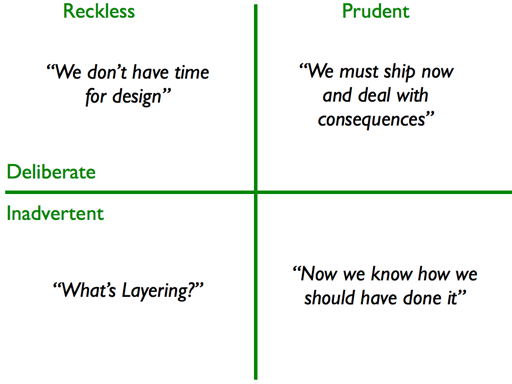
\includegraphics[width=80mm]{figures/chapter2/technicalDebtQuadrant}
	\caption{Technical Debt Quadrant}
	\label{fig:technical_debt_quadrant}
\end{figure}

\subsection{Other Insights on the Technical Debt Metaphor}

The technical debt metaphor has found favor with software developers who need to convey to project stakeholders uninitiated in programming terminology similar debts and patchwork repairs that ``kick the can down the road," temporarily delaying payment of money owed and putting off the effort of isolating a solution viable in the long term. Concepts falling under this umbrella include test and people debt, architectural and requirement debt and documentation and generalized software debt \cite{sterling2010managing}.

Broadening the metaphor to cover too many varieties of debt, however, might ultimately lessen its effectiveness, as Kruchten \textit{et al.} point out \cite{Kruchten_td_IEEE}.  Unimplemented requirements, functions or features do not qualify as requirement debts, just as putting off developing them does not qualify as a planning debt. Heavy reliance on tools alone to detect technical debt is one pitfall that the study highlights, in many cases leading to non-negligible underestimation of the actual technical debt load, since the majority of technical debt accumulates because of structural choices and technological gaps rather than code quality.

Further corroborating the overextension of the metaphor, Spinola \textit{et al.} \cite{spinola2013investigating} compiled statements on technical debt that software developers made both online and in published work and selected 14 of them to use as items in two surveys measuring the level of agreement of 37 participants with software development backgrounds. On the whole, most participants strongly agreed that poorly managed technical debt drives up maintenance costs until they outpace consumer value and disagreed that all technical debt is accrued with a developer's full knowledge.

In the same study, the authors speculate that the technical debt metaphor's comprehensibility is what fuels its generalization to phenomena outside the realm of technical debt in the truest sense. This in turn blurs the boundaries between technical debt and other costs or coding flaws and leads to persistent conflation among non-technical project contributors and, all too often, industry specialists, who adopt the metaphor as a rote catchall \cite{spinola2013investigating}.

Alves \textit{et al.}~\cite{alves2014towards} have introduced a specialized vocabulary intended to disambiguate the subtleties that an all-purpose term such as \textit{technical debt} overlooks, by sorting concepts extracted from a systematic literature mapping that combed 100 studies published between 2010 and 2014. Their undertaking identified 15 categories of technical debt but remained flexible enough to account for instantiations of technical debt that belonged in multiple categories: design debt, documentation debt, code debt, requirements debt, people debt, process debt, service debt, versioning debt, usability debt, build debt, test automation debt, infrastructure debt, defect debt, test debt and architecture debt. The work of Alves \textit{et al.} and others who have monitored trends in the application of the technical debt metaphor and devised schemata relaying its latest interpretations has allowed developers and their stakeholders to make sense of the dynamic interplay between holdover solutions and deferred expense.

\section{Technical Debt Indicators and Ramifications}


\subsection{Leveraging Source Code and Static Analysis Tools}

Lately, there has been a lot of incentive to engineer better strategies for detecting and managing technical debt. Technical debt often gets out of hand and reaches unsustainable levels because a developer neglects to take stock as it accumulates. For all their limitations, static analysis tools do efficiently pinpoint violations of object-oriented design principles and source code anomalies outside the pre-specified ranges quantifying code quality. Such outliers constitute ``bad smells," which fall under the category of design debt.\\

In a study probing the effects of god classes (another manifestation of design debt) on project maintainability, Zazworka \textit{et al.}~\cite{zazworka2011investigating} examined two commercial applications released by a development company and concluded that god classes are more liable to be defective, and thus higher-maintenance, than non-god classes. For this reason, it is worthwhile for developers to monitor and, where appropriate, rein in the toll that technical debt takes on product quality, at all stages in the process.\\

God classes and other bad smells---namely, data class and duplicate code---were extracted from open-source systems and scrutinized by Fontana \textit{et al.}~\cite{fontana2013code} in an effort to prioritize the handling of different types of design debt. Their approach ranks bad smells in descending order with respect to negative impact on software quality and encourages developers to rectify higher-priority design debts first.\\

Zazworka \textit{et al.}~\cite{zazworka2011investigating} elicited an enumeration of technical debt items stored in project artifacts from multiple developers and compared the results with what three static analysis tools identified as fitting the relevant criteria. As different teams reported different technical debt items, consensus engenders underestimation of the actual technical debt load and aggregation proves to be the better method. Similarly, static analysis tools  will yield underestimations---some varieties of technical debt going undetected---unless supplemented with human mediation.

\subsection{Leveraging Source Code Comments (Self-Admitted Technical Debt)}

While strides have been made in locating sources of technical debt and preventing unsustainable accumulation, such as integrating tool- and developer-flagged code, new improvements are constantly proposed, debated and adopted for use alongside older, ``tried and tested" methodologies. One such improvement, from Potdar and Shihab~\cite{ICSM_PotdarS14}, enlists source code comments in isolating technical debt, the benefit of which is that the program developer \emph{confesses} the debt. At best, analysis tools can only \emph{suppose} debt on the basis of semi-arbitrary cutoffs and thresholds, and stop short of guaranteeing that an implementation is less than optimal, i.e., \emph{self-admitted technical debt}.\\

In their pioneer study capturing the state of the art in \SATD identification, Potdar and Shihab~\cite{ICSM_PotdarS14} extracted source code comments from five open-source projects and conducted manual inspections. The authors read and analyzed more than 100,000 comments and in the end isolated 62 different comment patterns that serve as reliable indicators of \SATD, most consisting of simple phrases along the lines of ``fixme," ``workaround," and ``this can be a mess." It was found that: (i) between 2.4\% and 31.0\% of the files analyzed contained these keywords, (ii) the bulk of the \SATD was introduced by more experienced developers and (iii) there is no correlation between time pressures or code complexity and the amount of \SATD.\\

Building on the groundbreaking work of Potdar and Shihab~\cite{ICSM_PotdarS14}, Bavota and Russo~\cite{bavota2016large} considered the growth and evolution of self-admitted technical debt across 159 projects and the effects this has had on software quality, and extracted upwards of 600,000 commits and two billion source code comments. They found that: (i) \SATD is diffused, averaging 51 occurrences per system, (ii) it accumulates over time as new occurrences pile up on top of ones which have not yet been corrected and (iii) the occurrences that are corrected have a mean lifespan of 1,000 commits in the system.


\subsection{Research Leveraging Source Code Comments}
\todo{too similar to the last subsection's title?}


A number of studies examined the usefulness/quality of comments and showed that comments are valuable for program understanding and software maintenance \cite{TakangGM96,tan07icomment,lawrie2006leveraged}. For example, Storey \emph{et al.}~\cite{Storey:2008} explored how task annotations in source code help developers manage personal and team tasks. Takang {\em et al.} \cite{TakangGM96} empirically investigated the role of comments and identifiers on source code understanding. Their main finding showed that commented programs are more understandable than non-commented programs. Khamis {\em et al.} \cite{Khamis:2010} assessed the quality of source code documentation based on an analysis of the quality of language and consistency between source code and its comments. Tan {\em et al.} proposed several approaches to identify code-comment inconsistencies. The first, called @iComment, detects lock- and call-related inconsistencies \cite{tan07icomment}. The second approach, @aComment, detects synchronization inconsistencies related to interrupt context \cite{acomment}. A third approach, @tComment, automatically infers properties from Javadoc related to null values and exceptions; it performs test case generation by considering violations of the inferred properties \cite{tcomment}.\\

Other studies have examined the co-evolution of comment updates as well as the reasons behind them. Fluri {\em et al.} \cite{fluri2007code} studied the co-evolution of source code and associated comments and found that 97\% of the comment changes are consistently co-changed. Malik {\em et al.}  \cite{malik2008understanding} performed a large empirical study to understand the rationale for updating comments along three dimensions: characteristics of the modified function, characteristics of the change, as well as the time and code ownership. Their findings showed that the most relevant attributes associated with comment updates are the percentage of changed call dependencies and control statements, the age of the modified function and the number of co-changed functions which depend on it. De Lucia {\em et al.} \cite{DeLucia2011} proposed an approach to help developers maintain source code identifiers and consistent comments with high-level artifacts. The main results of their study, based on controlled experiments, confirm the conjecture that providing  developers with similarity between source code and high-level software artifacts helps to enhance the quality of comments and identifiers.



Most relevant to our research is the work recently undertaken by Potdar and Shihab~\cite{ICSM_PotdarS14}, which uses source code comments to detect \SATD. Using the identified technical debt, they studied  how much SATD exists, the rationale for SATD and the likelihood of its removal after introduction. Another relevant contribution to our study is Maldonado and Shihab's \cite{MTD15p9}, as their work has also leveraged source code comments to detect and quantify different types of SATD. They classified SATD into five types:  design debt, defect debt, documentation debt, requirement debt and test debt. Ultimately, they concluded that  the  most common type is design debt, accounting for anywhere between 42\% and 84\% of a total of 33,000 classified comments.

Our study builds on prior work in~\cite{ICSM_PotdarS14,MTD15p9} since we use the comment patterns they produced to detect SATD. However, in a departure from these studies, we examine the relationship between SATD and software quality.


\subsection{Technical Debt}

Other work has focused on the identification and examination of technical debt. It is important to note that the technical debt discussed here is \emph{not} SATD: rather, it is technical debt that is detected through source code analysis tools. For example,  Zazworka {\em et al.} \cite{Zazworka:2013} attempted to identify technical debt automatically and then compared their automated identification with human elicitation. The results of their study outline potential benefits of developing tools and heuristics for the detection of technical debt. Also, Zazworka {\em et al.} \cite{zazworka2011investigating} investigated how design debt, in the form of god classes, affects software maintainability and correctness of software products. Their study involved two industrial applications and showed that god classes are changed more often than non-god classes and, moreover, that they contain more defects. Their findings suggest that technical debt may negatively influence software quality. Guo {\em et al.}~\cite{GuoSGCTSSS11} analyzed how and to what extent technical debt affects software projects by tracking a single delayed task in a software project throughout its lifecycle. As discussed earlier, the work by Potdar and Shihab \cite{ICSM_PotdarS14} is also related to our work, which differs from precedent primarily in that it focuses on SATD.


Our work differs from foregoing research by Zazworka {\em et al.}~\cite{zazworka2011investigating,Zazworka:2013} since we focus on the relationship between SATD (and not technical debt related to god files) and software quality. However, we believe that our study complements prior studies since it sheds light on the overall impact of SATD and, in particular, its ramifications for software quality.



\subsection{Software Quality}

A plethora of prior work has proposed techniques to improve software quality, the majority of this work having concerned itself with understanding and predicting software quality issues (e.g.~\cite{Zimmerman2008Springer}). Several studies have examined the metrics that best indicate software defects, including design and code~\cite{Jiang-promise-2008}, code churn~\cite{Nagappan-icse-2005} and process metrics~\cite{Moser-icse-2008,Rahman-icse-2013}.

Other studies have opted to focus on change-level prediction of defects. Sliwerski  \emph{et al.} suggested a technique known as SZZ to automatically locate fix-inducing changes by linking a version archive to a bug database \cite{Sliwerski-fse-2005}.   Kim \emph{et al.} \cite{Kim-tse-2008} used identifiers in added and deleted source code and the words in change logs to identify changes as defect-prone or not. Similarly,  Kamei \cite{Kamei-tse-2013} proposed a  ``Just-In-Time Quality Assurance''  approach to identify risky software changes in real time.  The findings of their study reveal that process metrics outperform product metrics in terms of identifying risky changes.

Our study leverages the SZZ algorithm and some of the techniques presented in the aforementioned change-level work to study the defect-proneness of SATD-related commits. Moreover, our study complements existing work by taking up the hypothetical correlation between SATD and software defects.
